%% Template for MLP Coursework 1 / 16 October 2017 

%% Based on  LaTeX template for ICML 2017 - example_paper.tex at 
%%  https://2017.icml.cc/Conferences/2017/StyleAuthorInstructions

\documentclass{article}

\usepackage[T1]{fontenc}
\usepackage{amssymb,amsmath}
\usepackage{txfonts}
\usepackage{microtype}
\usepackage{enumitem}
\usepackage{float}

\usepackage[utf8]{inputenc}
\usepackage{csquotes}

% For figures
\usepackage{graphicx}
\usepackage{subfigure} 

% For citations
\usepackage{natbib}

% For algorithms
\usepackage{algorithm}
\usepackage{algorithmic}
\usepackage[toc,page]{appendix}

% the hyperref package is used to produce hyperlinks in the
% resulting PDF.  If this breaks your system, please commend out the
% following usepackage line and replace \usepackage{mlp2017} with
% \usepackage[nohyperref]{mlp2017} below.
\usepackage{hyperref}
\usepackage{url}
\urlstyle{same}

% Packages hyperref and algorithmic misbehave sometimes.  We can fix
% this with the following command.
\newcommand{\theHalgorithm}{\arabic{algorithm}}


% Set up MLP coursework style (based on ICML style)
\usepackage{mlp2017}
\mlptitlerunning{MLP Coursework 4 (\studentNumber)}
\bibliographystyle{icml2017}

\DeclareMathOperator{\softmax}{softmax}
\DeclareMathOperator{\sigmoid}{sigmoid}
\DeclareMathOperator{\sgn}{sgn}
\DeclareMathOperator{\relu}{relu}
\DeclareMathOperator{\lrelu}{lrelu}
\DeclareMathOperator{\elu}{elu}
\DeclareMathOperator{\selu}{selu}
\DeclareMathOperator{\maxout}{maxout}

%% You probably do not need to change anything above this comment

%% REPLACE this with your student number
\def\studentNumber{s1700260, s1457374, s1784849}

\begin{document} 

\twocolumn[
\mlptitle{MLP Coursework 4: Project Final Report \\
Transfer learning and dataset size - Group G74
}

\centerline{\studentNumber}

\vskip 7mm
]

\begin{abstract} 
Following from our previous research, we initially re-orientate the reader by re-introducing and expanding upon the research topics that are explored pertaining to transfer learning. Furthermore, the findings from the interim report are summarised, and our research questions and hypotheses are stated. The investigated domains are related to three fundamental research questions. Firstly, how can transfer learning be used to improve the performance of image classification tasks when the availability of data is limited. Secondly, how viable is a modified Siamese neural network, inspired by \cite{koch}, combined with transfer learning to accomplish the aforementioned goal. Finally, how does perceived visual similarity between datasets affect the performance of transfer learning. We found that transfer learning is effective when dealing with small data, but it may also be suggested that the benefits of transfer learning depend on the characteristics of the target dataset. Some success was achieved using the modified Siamese neural network, but we believe additional work is required in this space to make further progress.
\end{abstract} 

\section{Introduction}
\label{sec:intro}

Large-scale neural networks have become increasingly prevalent in artificial intelligence \cite{krizhevsky2012imagenet}. Such architectures effectively solve computer vision problems that were previously considered difficult to address using traditional symbolic manipulation \cite{dinsmore2014symbolic}. One concern with modern neural networks is that their performance scales with the quantity of data used to train them \cite{interim-report}. This concern is a problem for individuals or institutions with small amounts of data that want to implement these architectures as solutions, or for research purposes.

Data-driven techniques exist, such as data augmentation \cite{krizhevsky2012imagenet}, which help solve this problem. However, to draw from our previous research \cite{interim-report} we investigate alternative, machine learning based approaches. Specifically, transfer learning \cite{oquab2014learning}, \citep{ng2015deep}, \citep{chen2016deep} as methods to improve the performance of neural network architectures that utilise small amounts of data. These techniques allow us to use the knowledge that a given (pre-trained) network already has and adapt the architecture to suit our requirements.

The objective of transfer learning is to use the knowledge acquired by an existing network that was built to solve a similar task to improve the generalisation of a novel task. A significant advantage of utilising this technique is that the neural network model does not have to learn from scratch. Prior learning (computational work) can be re-utilised which is essential when the resources are limited, which is significant for convolutional neural networks, which, depending on the size of the architecture, can require a considerable amount of computational power.

Numerous pre-trained neural networks to solve classification tasks exist in the field of computer vision. One of them is the Visual Geometry Group network (VGG net) \cite{DBLP:journals/corr/SimonyanZ14a}. This network implements a simple yet deep architecture with several convolutional layers. There are several configurations that vary the number of convolutional layers among 11, 13, 16, and 19. In every configuration the architecture includes maximum pooling layers of dimensions 2x2 and stride 1. The convolutions are performed using 3x3 filters with stride and pad of 1. Finally, ReLU activations after each convolution are utilised.

VGG net was first used in the ImageNet Challenge 2014 \cite{DBLP:journals/corr/SimonyanZ14a}, which means that is was originally trained using the Imagenet dataset \cite{deng2009imagenet}. However, the network has also been trained in other datasets like CIFAR-10 \cite{krizhevsky2014cifar} and CIFAR-100 \cite{CIFAR-100}. It is important to make this distinction since each dataset has been developed for a different purpose. Therefore, they have specific characteristics. The knowledge learnt from a network depends on the dataset used to train it. Thus, it is critical to know the characteristics of the dataset utilised to train the network since it will play an important role when implementing transfer learning.

ImageNet is a large-scale hierarchical image database \cite{ImageNet}. The structure of this dataset contains 12 main groups or sub-trees. Each sub-tree contains a variable number of categories. The total number of categories is 5247, each one containing on average 600 images, thus, the total number of images in the dataset is 3.2 million. As described, ImageNet is a large and diverse dataset. However, the original version of VGG net was trained on a subset of Imagenet that contains only 1000 categories using 1.3 million images for training, 50K images for validation and 100K images for testing.

\subsection{Interim Report Findings}
\label{sec:findings}

The research questions offered within this report have been drawn from our initial findings, as documented in the interim report \cite{interim-report}. To aid in orientating the reader, we provide a summary of these findings here.

It was possible to demonstrate how the amount of available data impacts the performance of a convolutional neural network. Such impact was observed in the validation stage by analysing the accuracy and error of the network. In the first case, it was evident the reduction of the accuracy as the size of the dataset was reduced. In the second case, the size of the dataset directly affected the error; the smaller the dataset, the bigger the error. In both cases, the ultimate effect of such behaviour was the difficulty of the network to generalize when the amount of data is small.

Furthermore, the usage of two different but comparable databases provided some extra insights about the behaviour of the neural network. In this case, the observed accuracies in the validation stage were different for each dataset in every size used to train the network. Under these circumstances, it was clear that the dataset that allowed a higher accuracy (clothes) was less challenging for the network. This means, that the features extracted by the network were more useful and relevant for one of the datasets. In the other hand, the features learned by the network did not provide enough information to reach better results for the second dataset (expressions).

Finally, we demonstrated that a simple data-driven technique like data augmentation effectively improves the performance of a simple convolutional neural network. However, the benefits of this method have a limit above which no further improvement can be done. All of these findings provided the foundations and motivation for our investigation.

\section{Objectives and Research Questions}
\label{sec:obj_questions}

\subsection{Objectives}
\label{sec:objectives}

There are two fundamental objectives. The first one concerns with improving the performance of the image classification task using transfer learning under conditions of small data. The second objective investigates the effects of transfer learning on two distinct but comparable datasets.

\subsection{Research Questions}
\label{sec:questions}

Following from the conclusions drawn from our interim report, our research questions are listed below.

\begin{enumerate}
  \item How much the performance for a given classification task can be improved by using transfer learning?  
  \item How much the application of transfer learning affect two distinct but comparable datasets?
\end{enumerate}

\subsection{Hypotheses}
\label{sec:hypotheses}
\begin{enumerate}[label=\textbf{H.\arabic*}]
  \item \label{h:1} Transfer learning will provide a performance benefit with respect to the generalisability (measured through validation accuracy) for the given classification task in conditions of small data.
  \item \label{h:2} Transfer learning will provide a larger performance boost when the size of the dataset used to initially train the model is small rather than large.
\end{enumerate}

\section{Methodology}
\label{sec:methodology}

\subsection{Simple Transfer Learning}
\label{sec:transferlearninng}

\subsubsection{\textbf{Chosen Model}}

We decided to select the VGG net configuration with 16 convolutional layers (hereinafter referred as VGG16) to transfer its knowledge into the clothes and expressions datasets. As previously mentioned, this network is quite simple and deep; thus, the expectation is that the knowledge contained in this network will be sufficient to increase the generalisability of the classification tasks using both datasets.

Since the available versions of VGG16 have been trained with different datasets, we decided to use the knowledge obtained from ImageNet rather than other options like CIFAR- 100. The main reason for this decision is the number of classes from the subset of ImageNet to train the network (1000) which is much bigger than the number of classes from CIFAR-100 (100). The expectation is that the knowledge from ImageNet is more extensive, therefore, it can provide better results when transferring that knowledge into new datasets.

\subsubsection{\textbf{Configuration}}

The configuration to adapt the knowledge from VGG16 into the current task is made of two stages. The first one consists of extracting part of the knowledge from VGG16. One of the primary interests is to extract a sufficient number of relevant features to increase the generalisation for the classification task. This situation can be accomplished by using the knowledge from the convolutional layers. The second part consists in the adaptation of the extracted knowledge. This goal is achieved by discarding the original fully connected layers of VGG16. Then, a new set of fully connected layers adapted for the current task are implemented. Thus, the configuration is made of the convolutional layers from VGG16 connected to custom fully connected layers adapted for the current classification task.

The described configuration has a bottleneck between the convolutional layers and the fully connected ones. This bottleneck is caused by the number of convolutions that has to be done in every layer which requires a considerable amount of computational power. To reduce the impact of the described bottleneck the transfer learning is divided into two phases.

In the first phase, only the convolutional layers are utilised. The knowledge obtained from these layers is not modified. That means that their parameters from those layers are not updated while using the clothes and expressions datasets. Under these circumstances, the images from the datasets are passed through the convolutional layers, and the output from the last one is stored for the second phase.

This process can be seen as a feature extraction stage. The raw images are converted from their original representation to a new one. The original representation of the images provides information about the pixel intensity. After passing the images through the convolutional layers, the pixel intensity information is converted to other of type of information based on the local spatial correlation of the pixels which is obtained with the convolutions.

The process of converting the images from their original representation to another using convolutional layers is computational expensive. However, one of the benefits it provides is the dimensionality reduction of the representation of the images. Each input image is converted from a representation of 4096 (64x64) pixel intensities to a representation of 2048 new features. This means a reduction in the dimensionality of the images of 50\%.

In the first option, only one fully connected layer is defined. This option provides 205,607 trainable parameters. The second alternative adds another fully connected layer on top of the one from the first option. The total number of parameters for this alternative 210,307 parameters. For the final alternative, a new fully connected layer is added on top of the previous ones. The final number of parameters for this option is 211,407.

In every set of fully connected layers, an L2 regularisation strategy is used. The primary objective of this strategy is to reduce the chances of overfitting, which is especially crucial for small data. Each layer uses a uniform parameter initialisation strategy. This kind of initialisation allows having the activation done in the plateau region of a sigmoid function. Non-linear activation functions are added following the convolutional layers. For the output layer, a softmax activation with a categorical cross entropy error loss is implemented. The implemented learning rule is Adam.

\subsection{One Shot Learning and Transfer Learning by Learning Similarity}
\label{sec:oneshot}

\subsubsection{\textbf{Siamese Neural Network}}

We are interested in using an alternative transfer learning method to solve the problem of insufficient target data for training. We suggest that this may be accomplished using a methodology inspired by \cite{koch}\footnote{We would utilise a Siamese-like network to perform a similar operation to one-shot learning tasks} to learn to distinguish between images (using a similarity metric) from a related training dataset that differs from the target dataset. Moreover, they also transferred the learnt similiarity metric to classify classes from the MNIST set and achieved $70\%$ accuracy. This methodology differs from the previously proposed method \ref{sec:transferlearninng} since the training data would be different (but related to) the target data, to be classified.

In the original paper, Koch et.al first trained on subclasses of and tested on other unseen classes of the Omniglot dataset (a character dataset similar to MNIST). The Siamese network consisted of numerous convolutional layers that implement the ReLU activation function, followed by max-pooling layers, followed by fully connected layers and an L1 distance layer. This architecture allows for learning of generic features in images and provides a similarity metric between image pairs.

In this project, we propose an augmented version of the Siamese network as is suggested in the original paper. Since training convolutional layers could allow the neural network to learn general features of images, replacing the convolutional layers with part of the VGG16 (transfer) architecture may enable a more accurate similarity metric to be output. We assume a higher accuracy in similarity because VGG16 has already learnt an abundance of knowledge (regarding feature representation). Transfering VGG16 into the Siamese architecture also suggests that there is far less training required, as we would hope it would be easier to tune than train from scratch.

\section{Experiments}
\label{sec:experiments}

\subsection{Simple Transfer Learning}

\subsubsection{\textbf{Motivation}}

Transfer learning is a technique that takes advantage of previous work. The objective is to adapt that prior work to the specific circumstances of a similar new problem. As demonstrated in the previous research, the size of the dataset has a direct impact in the performance of a neural network. Therefore, the experiments of this new research are aimed to evaluate the benefits of transfer learning under the conditions of small data.

\subsubsection{\textbf{Description}}

Based on the prior findings of the existence of a correlation between the available data and the performance of a neural network, the experiments are mainly focused in the behaviour of the proposed approach for different sizes of the datasets. Even though the primary focus is on small data, the evaluation of the proposed approach is executed over other sizes to obtain a greater insight in relation the performance of the solution as the data is scaled down. Therefore, each experiment was conducted using the following dataset sample sizes: 100\%, 10\%, 1\%, 0.1\%. To ensure empirical comparisons of the validation accuracy the number of samples at every stage is kept constant for every experiment as seen in Tables \ref{tab:ds_1} and Table \ref{tab:ds_2}.

\begin{table*}[!htb]
  \centering
  \begin{tabular}{| l | l | l | l | l |}
    \hline
    \textbf{Size} & \textbf{Training samples} & \textbf{Training samples per class} & \textbf{Validation samples} & \textbf{Validation samples per class} \\ \hline
    100\% & 42000 & 6000 & 7000 & 1000 \\ \hline
    10\% & 4200 & 600 & 7000 & 1000 \\ \hline
    1\% & 420  & 60 & 7000 & 1000 \\ \hline
    0.1\% & 42 & 6 & 7000 & 1000 \\ \hline
  \end{tabular}
  \caption{Number of samples for each size of the clothes dataset.}
  \label{tab:ds_1}
\end{table*}  
  
\begin{table*}[!htb]
  \centering
  \begin{tabular}{| l | l | l | l | l |}
    \hline
    \textbf{Size} & \textbf{Training samples} & \textbf{Training samples per class} & \textbf{Validation samples} & \textbf{Validation samples per class} \\ \hline
    100\% & 42000 & 6000 & 6300 & 900 \\ \hline
    10\% & 4200 & 600 & 6300 & 900 \\ \hline
    1\% & 420  & 60 & 6300 & 900 \\ \hline
    0.1\% & 42 & 6 & 6300 & 900 \\ \hline
  \end{tabular}
  \caption{Number of samples for each size of the expressions dataset.}
  \label{tab:ds_2}
\end{table*}

To search for a practical set of system parameters, we decided that varying the activation functions at every fully connected layer would be interesting to explore. It follows that each experiment was initially performed using a standard sigmoid function \cite{hecht1992theory}. The selection of this function was to obtain the benefits of a uniform initialisation strategy. However, we also ran each experiment using exponential linear units (ELU) \cite{clevert2015fast}. This activation enables other kinds of non-linearities. The main advantage of implementing ELU is its gradient which is similar to the natural gradient (smooth). Finally, we also performed a manual sensitivity analysis by varying the learning rate values from the follow pool: 0.01, 0.001, 0.0001.

Based on the description of the components in the methodology for the transfer learning approach, we configured the experiment using three sets of fully connected layers, two different types of activation functions, four dataset subsamples and a pool of three different learning rates. Combinations of the above result in 72 different experiments for each dataset. Due to the amount of experiments and the limited computational resources, we set a fixed number of epochs for every experiment (20), and a fixed size for the mini-batches used for the stochastic gradient descent calculation (50).

After running the aforementioned experiments, we analysed the results based on the validation accuracy. Then, we selected the configurations that get the highest values for validation accuracy for dataset sizes of 1\% and 0.1\%. For further investigation we then performed new experiments with higher number of epochs (200) to analyse the behaviour of the fully connected part of the architecture under conditions of small data.

\subsubsection{\textbf{Results}}

In order to compare the results of the current experiments to the baselines described in the previous report, the analysis of the transfer learning experiments is focused on the validation accuracy. Overall, there is still an evident reduction of the performance of the architecture related to the size of the datasets, as shown in Figure \ref{fig:tf_clot} and Figure \ref{fig:tf_exp}.

\begin{figure*}
  \vskip 5mm
    \begin{center}
      \minipage[scale=0.8]{0.45\textwidth}
        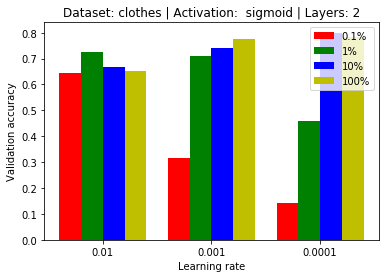
\includegraphics[scale=0.45]{accuracy_reduction_00.png}
        \caption{Validation accuracy comparison for the clothes dataset. The configuration with two fully connected layers and Sigmoid activations allows the highest accuracy for the smallest size of the dataset.}
        \label{fig:tf_clot}
      \endminipage\hfill
      \minipage[scale=0.8]{0.45\textwidth}
        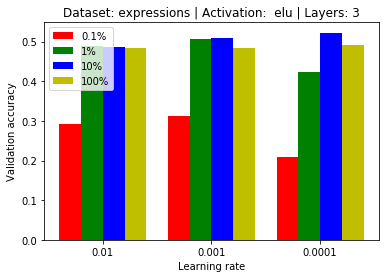
\includegraphics[scale=0.45]{accuracy_reduction_01.png}
        \caption{Validation accuracy comparison for the expression dataset. The configuration with three fully connected layers and ELU activations allows the highest accuracy for the smallest size of the dataset.}
        \label{fig:tf_exp}
      \endminipage\hfill
    \end{center}
  \vskip -5mm
\end{figure*}

%\begin{figure*}
%   \vskip 5mm
%        \begin{center}
%            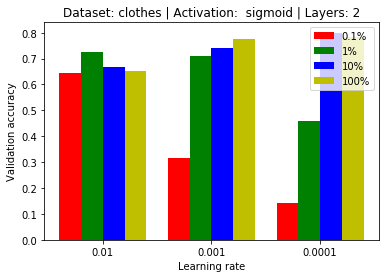
\includegraphics[scale=0.5]{accuracy_reduction_00.png}
%            \caption{Validation accuracy comparison for the clothes dataset. The configuration with two fully connected layers and Sigmoid activations allows the highest accuracy for the smallest size of the dataset.}
%            \label{fig:tf_clot}
%        \end{center}
%    \vskip -5mm
%\end{figure*}

%\begin{figure*}[tb]
%    \vskip 5mm
%        \begin{center}
%            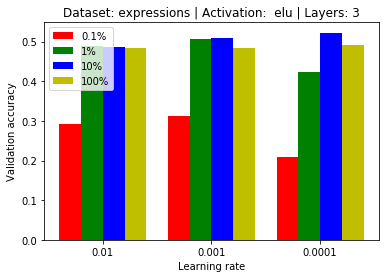
\includegraphics[scale=0.5]{accuracy_reduction_01.png}
%            \caption{Validation accuracy comparison for the expression dataset. The configuration with three fully connected layers and ELU activations allows the highest accuracy for the smallest size of the dataset.}
%            \label{fig:tf_exp}
%        \end{center}
%    \vskip -5mm
%\end{figure*}

Figure \ref{fig:tf_clot} shows the effect of the learning rate for every size of the clothes dataset. It is evident how differently the hyper-parameter affect the validation accuracy of the system for each size. While the learning rate reduces, the validation accuracy when the sizes are 0.1\% and 1\% increases. In the other hand, the increase of the learning rate reduces the validation accuracy when the sizes are 10\% and 100\%. This behaviour might be an indicator of the relationship between the number of available training samples and the learning rate when the batch size is kept constant.

Figure \ref{fig:tf_exp} shows the effect of the learning rate for every size of the expressions dataset. Similarly, the size of the learning rate has a positive impact for small sizes, and a negative one for bigger sizes. However, the validation accuracy is reduced for small sizes when the learning rates goes from 0.001 to 0.01. The increase in learning rate may suggest the existence of a peak where the benefits of a high degree of learning for small sizes starts to decrease.

For each dataset, the configurations that provides the highest accuracy for the smallest dataset size are quite different, as seen in Table \ref{tab:tf_1}. It is especially important to take note of the activation functions. It is expected that the Sigmoid activation function will yeild better results since the uniform initialisation strategy is meant to benefit this activation function. However, in the case of expressions dataset, the best result is obtained with ELU, but the best accuracy using Sigmoid activations is not that far (0.30).

\begin{table*}[!htb]
  \vskip 5mm
  \centering
  \begin{tabular}{| l | l | l | l | l |}
    \hline
    \textbf{Dataset} & \textbf{Validation accuracy} & \textbf{Fully connected layers}& \textbf{Activation} & \textbf{Learning rates}\\ \hline
    Clothes & 0.64 & 2 & Sigmoid & 0.01 \\ \hline
    Expressions & 0.31  & 3 & ELU & 0.001 \\ \hline
  \end{tabular}
  \caption{Configuration that allows the highest accuracy for size of 0.1\% for clothes and expressions datasets}
  \label{tab:tf_1}
\end{table*}

\begin{table*}[!htb]
  \centering
  \begin{tabular}{| l | l | l | l | l | l |}
    \hline
    \textbf{Dataset} & \textbf{Size} & \textbf{Baseline} & \textbf{Data Augmentation}& \textbf{Transfer learning} \\ \hline
    Clothes & 1\% & 0.50 & 0.76 & 0.75 \\ \hline
    Clothes & 100\% & 0.51 & 0.76 & 0.78 \\ \hline
    Expressions & 1\% & 0.32  & 0.44 & 0.50 \\ \hline
    Expressions & 100\% & 0.34  & 0.49 & 0.50 \\ \hline
  \end{tabular}
  \caption{Validation accuracy for baseline system, data augmentation, and transfer learning when dataset sizes are 1\% and 100\%}
  \label{tab:tf_2}
\end{table*}

\begin{table*}[!htb]
  \centering
  \begin{tabular}{| l | l | l | l |}
    \hline
    \textbf{Dataset} & \textbf{Size} & \textbf{RG} &\textbf{AG} \\ \hline
    Clothes & 1\% & 1.5 & 0.25 \\ \hline
    Clothes & 100\% & 1.52 & 0.27 \\ \hline
    Expressions & 1\% & 1.56 & 0.18 \\ \hline
    Expressions & 100\% & 1.47 & 0.16 \\ \hline
  \end{tabular}
  \caption{Relative and absolute gain when dataset sizes are
1\% and 100\%.}
  \label{tab:tf_3}
\end{table*}

As seen in \ref{fig:tf_beh}, the behaviour of the system for the smallest sizes is stabler for the clothes than for the expressions. In the case of the clothes dataset, for 1\% and 0.1\% of the original size, the system reaches a point where it starts to overfit. However, it is noticeable how the configuration of the system is robust enough to try to minimise overfitting. Evidently, the number of available images play an important role in the reduction of the error. The minimum validation error of 0.1\% is reached around the 30\textsuperscript{th} epoch. For 1\%, the minimum validation error is reached around epoch number 50.

In the case of the expressions dataset, the behaviour of the system is completely distinct not just compared to the clothes, but between the sizes of the dataset. For 1\% of the size, the configuration of the system is not robust enough to minimise the effects of overfitting. Once the overfitting starts, the efforts of the system to reduce it are not enough. However, for the case of 0.1\%, the configuration of the system seems to be robust.  At first, the overfitting effect is dramatic, then it reaches a point where the system starts to recover from it. The recovery is a long process where the system tries to learn from the training set. Eventually, the system reaches a point where the recovery is stopped and the overfitting starts again.

\begin{figure*}[tb]
    \vskip 5mm
        \begin{center}
            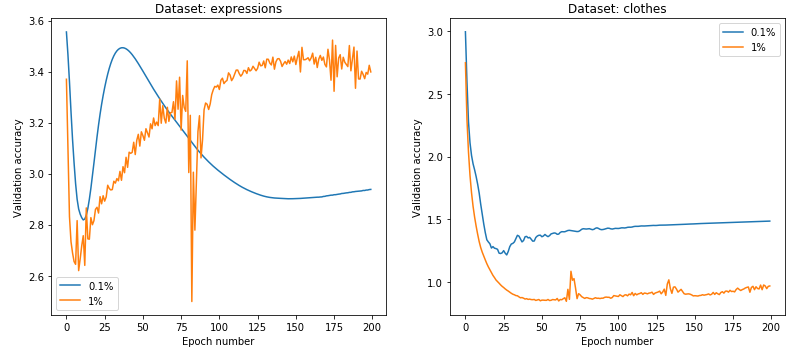
\includegraphics[scale=0.375]{behaviour_rotated.png}
            \caption{Comparison of the evolution of the validation error when the sizes of the datasets are 1\% and 0.1\%. The effects of over-fitting are clearly more dramatic for expressions that for clothes. The system presents a better behaviours when classifying clothes. }
            \label{fig:tf_beh}
        \end{center}
    \vskip -5mm
\end{figure*}

\subsubsection{\textbf{Interpretation and Discussion}}

The proposed system provides some benefits when the number of samples in the datasets is small. Depending on the context of analysis, these benefits can be higher for one dataset or the other. At first, transfer learning seems to be more effective for the clothes dataset than for the expressions dataset as seen in Figure \ref{fig:tf_clot} and Figure \ref{fig:tf_exp}. This information provide an indication regarding the complexity of the images in every dataset. At a glance, the experimental results allows us to suggest that the features extracted from the clothes are less challenging to learn than those extracted from the expressions.

\begin{equation}
	RG = \frac{Val\ Acc_{tranfer\ learning}}{Val\ Acc_{baseline}}
	\label{eq:eq1}
\end{equation}

	


\begin{equation}
	AG = Val\ Acc_{tranfer\ learning} - Val\ Acc_{baseline}
	\label{eq:eq2}
\end{equation}

% work around for getting footnotes in tables, see: https://tex.stackexchange.com/questions/1583/footnotes-in-tables

%\addtocounter{footnote}{-2}
%\footnotetext[2]{RG for Relative gain.}
%\addtocounter{footnote}{1}
%\footnotetext[3]{DA for data augmentation.}
%\addtocounter{footnote}{1}
%\footnotetext[4]{AG for absolute gain.}

% end of workaround

A further analysis requires to compare the validation accuracy between transfer learning and the baseline system. Two relations help to better understand the benefits of transfer learning. The first is relative gain, defined as the ratio between the validation accuracy from transfer learning and the validation accuracy from the baseline system as seen in expression \ref{eq:eq1}. The second relation is absolute gain, defined as the difference between the validation accuracy from transfer learning and the validation accuracy from the baseline system as seen in expression \ref{eq:eq2}.

The use of the previous relations allows us to state that the knowledge obtained by VGG16 from the ImageNet dataset was more beneficial for the expressions dataset in terms of relative gain. The relative gain values are 1.5 and 1.56 for the clothes and expressions dataset respectively. This might indicate that VGG16 extracted features that were more relevant for expressions rather than for clothes.

In terms of absolute gain, the knowledge from VGG16 was more beneficial for the clothes dataset. The additional validation accuracies obtained from transfer learning compared to the baseline system were 0.25 and 0.18 for the clothes and expressions dataset, respectively, as seen in \ref{tab:tf_3}. Even though the extracted features from VGG16 could have been more relevant for expressions, they were good enough to increase the performance of the system for clothes.

However, comparing the results of transfer learning with the ones obtained from data augmentation, we see that the values are dispair as seen in \ref{tab:tf_2}. The validation accuracy is almost the same for the clothes dataset when the size is 1\% . For expressions, the difference is higher, 0.44 for data augmentation and 0.50 for transfer learning.Therefore, the benefits of data augmentation are comparable to the benefits of transfer learning for the clothes dataset. One possible explanation is in the kind of information obtained from images.

Convolutional layers extract information about the local spatial correlation of images. The result of this process is the detection of edges, shapes, patterns and other geometric information. The baseline system was shallow and only contained one convolutional layer. Thus, the geometric information extracted from this single layer along with data augmentation provided enough elements to increase the performance in the classification task in a way that it was comparable to the benefits obtained from transfer learning. 

When comparing the benefits of transfer learning under the conditions of low and high number of samples, the results are dis-pair. First, the benefits are higher when the number of clothes samples is higher as seen in \ref{tab:tf_3}. The relative and absolute gains are higher when using 100\% of the clothes dataset. In the other hands, the benefits are higher when the number of expressions samples is lower. The relative and absolute gains are higher when using only 1\% of the expressions dataset.

\subsection{Siamese Neural Network}

\subsubsection{\textbf{Description and motivation}}

Our model consists of first 19 layers in VGG16 followed by a flatten layer which converts all features from the previous layers to
an equivalent n-dimensional matrix (n,) in python. These vectors are then passed to a fully connected layer with sigmoid activation which outputs 4096 vectors. Next, we pass these vectors to our defined L1 distance layer which calculates the L1 distance between pairs of input images as a scalar. Finally, we output the probability of each pair of images being in the same class separately based on a last fully connected layer, also with a sigmoid activation. Binary cross-entropy is therefore used as the loss function.

To train the entire network, we freeze the first 19 layers from VGG16 to encapsulate both generic and detailed features of images learnt by VGG16 while training remaining layers to ensure that the network is learning according to inputs. To avoid overfitting, we utilise L2 regularization with $\lambda=0.0001$. Since the original paper used different and decaying learning rates in each layer, adopting such approach on VGG16 would be difficult. We therefore simplified to use the Adam learning rule with a learning rate 0.001 as we have observed that choices of learning rule/rate doesn't seem to affect much on the prediction accuracy.

\subsubsection{\textbf{Experimental setup}}

The goal is to train our VGG16-augmented Siamese Network to classify unseen classes of images by learning to distinguish similarity between images. The input is in terms of N pairs of image each having (64,64,3) matrix encoded as pixels. As in the original paper, each of the two twin images in every pairs of images are passed to the model separately with weight sharing. This is to ensure symmetric invariance in model, such that L1 distance layer output the same distance when the order of the two twins image inputted is changed. This is done by merging two twins to the L1 distance layer $|\phi(first twin) - \phi(second twin)|$ where $\phi$ is the flattened output from VGG16 and input of the entire network takes the form $pairs = [first twin,second twin]$. First twin and second twin has input shape (batch size,64,64,3). The batch size determines no. of pairs to be trained during each epoch. As suggested in the original paper, we also ensure 50$\%$ of same and different class are used in pairs and randomly sampled among $k$ available images in each classes. For the training data, we used first three catagories of the animated facial expression dataset (42k images in 7 classes), as seen in \ref{appendix:face-ds}, and japanese female facial expression dataset (203 in 7 classes), as seen in \ref{appendix:jap-ds}, in two separate runs. Both of the dataset also contains 7 classes of expression.

In the first approach, both training and test data are animated facial expression dataset. However, we only included the first three catagories during training and the 4 unseen class during test time. This is to test the effectiveness of the proposed model on predicting unseen images but with a softer restriction. The model is allowed to learn representation on subset of classes of the target dataset but tested on other unseen classes of the same dataset. Note that this approach is still distinct from standard machine learning procedure as training is not directly on same kind of target dataset. Among the three catagories, we randomly sampled 36 pairs of images randomly sampled from 900x3 available images from 3 classes in each epoch training. It is also ensured that 50$\%$ same and different classes are drawn.

In the second approach, restriction is increased and allow only related but entirely different dataset (Japanese female dataset) for training. There are in total 29x7 images in 7 catagories. Apparently, the size of dataset is too few comparing to dataset in first approach. The reason of using this dataset is due to limited availability of grayscale facial expression dataset from internet and this is the only dataset that shares most geometric similarity with the target set(animated facial expression), as location, classes and placement angles are most similar comparing to other datasets such as extended cohn-kanade facial dataset.

\subsubsection{\textbf{Results}}

In the first approach, training accuracy increases for first 50 epoch training ranging from $49-68\%$ which proves that the model is in fact learning. During test time, 320 one shot learning tasks is performed after epochs of training. In each one shot learning task,6 different and 1 same class pairs of image is randomly drawn from 6000x4 images. If the model successfully predicts the pair, we add one to accuracy, the overall accuracy is then calculated in terms of $(100.0)x( no.of.correct )/ 320$. At 1st epoch, accuracy is around $28\%$ which is close to random guessing. At 20th epoch, accuracy reaches $40-49\%$ for several runs of the 320 one shot task and doesnt improve further for more epochs. In second approach, we used 96 and 198 batch size in training to allow more learning and test if overfitting would occur. Moreover,similar 320 one shot learning tasks are performed to classify 7 unseen catagories from pairs randomly drawn from 6000x7 images. For 96 batch size after 50th epoch of training, test accuracy ranges from $22.8125-28.4375\%$. For 198 batch size, test accuracy falls in range of $20-30\%$. Overfitting seems not to be occured as increasing batch size for training does not affect much on test accuracy.

\subsubsection{\textbf{Interpretation and Discussion}}

For the first approach, we achieved best test accuracy of $50\%$. This might be because training set shares generic features on hairstyle,shape of face, sexuality of characters with target set. However, the result also showed effectiveness of using similarity differences to classify unseen images as we have not trained the network to learn about the other 4 expressions.

Note that in both of the approaches, test accuracy is better than random guessing by $~100\%$ which suggests accuracies measured are not due to randomization. In the second approach, test accuracy drops significantly which is probably due to insufficient training set. Moreover, there are greater differences between training and target set than in first approach. Given more available dataset and time, it is expected that the second approach would achieve better results. Another reason of the performances could be attributed to use of grayscale images. Since VGG16 trained on RGB images, weights in the network are trained to learn colorful images. Using grayscale images would alter performances of VGG16. Overall, results have shown that our model demonstrated the ability to predict unseen images by transferring representation of related but different images to solve one shot learning tasks, to preliminary extent.

\section{Related work}
\label{sec:related}

In order to place our research in a wider context, we offer a brief review of published work that that has been foundational in our efforts to explore the implications of using small data on convolutional neural networks. Initially, our research associated with small data was inspired by a quote from Andrew Ng from an article on nanonets \cite{nanoNets}:

\begin{displayquote}
I think AI is akin to building a rocket ship. You need a huge engine and a lot of fuel. If you have a large engine and a tiny amount of fuel, you won’t make it to orbit.
\end{displayquote}

Further, understanding how much data one may require to obtain a satisfactory level of performance on image classification problems seemed to be an interesting proposition \cite{howMuchData}. 

Additional motivation for investigating transfer learning was to take advantage of previous work (training), one benefit of this approach is the saving of computational resources. Some available pre-trained networks for vision tasks have been developed by feeding them several million of images and using a considerable amount of computational resources. These resources are not available for every organization, institution or individual.

After reviewing other papers such as \cite{NIPS2014_5347} and \cite{oquab2014learning}, we found that transfer learning is a versitile method to reduce training time and data required, especially when dealing with low level representations \cite{NIPS2014_5347}. Other experiments on small dataset have made comparisons between shallow and deep architectures to minimize the effects of overfitting \citep{pasupa2016comparison}. The results of these experiments statistically demonstrated that shallow models did perform better than deep ones with no regularization. However, a combination of various regularization techniques increased the performance of the deep models. As described in the configuration of the simple transfer learning in this report, the use of regularization techniques did provide some robustness to cope with overfitting as seen in Figure \ref{fig:tf_beh}.

One academic paper that investigates transfer learning in the context of small data includes \citep{ng2015deep}. This project tried to adapt the knowledge from a convolutional neural network trained on ImageNet to a classification task related to the recognition of facial expressions using two new datasets. The approach implemented by the authors included a cascade fine-tuning methodology where the pre-trained network was first adapted to one dataset, then a further adaptation was performed using the second dataset. The best validation accuracy in their experiments was 0.49, close to 0.50 presented in this report. This result could confirm the level of complexity to classify facial expressions.

Inspired by the paper as mentioned above, we thought it would be interesting to investigate how distinctly different (but comparable) datasets (with a large difference between the degrees of perceived visual similarity between classes) perform agaisnt one another in image classification tasks that utilise transfer learning. This in and of itself is an interesting research domain because the notion of perceived visual similarity has only recently began being explored within the literature. Consequently, we decided to consider methods which could compute similarity metrics for measuring the difference between classes and datasets. As one-shot learning tasks, such as person re-identification \cite{ahmed2015improved} performs similar roles (by passing some similarity metric through a threshold function), we began to explore the literature related to siamese convolutional networks \cite{koch}.

Further work can be aimed to investigate the effects of transfer learning in combination with data augmentation for small data. As seen in Table \ref{tab:tf_2}, the accuracy gain of transfer learning and data augmentation are comparable, especially for clothes. A combination of both approaches could potentially increase the performance of the model more than using them independently. Additional future work could build upon the aforementioned apporach to measuring perceived visual similarity between datasets and the effect that this has on positive and negative transfer.

\section{Conclusions}
\label{sec:conclusions}

\subsection{Transfer Learning}

As per the results of the experiments presented previously, there are two main conclusions in regards to transfer learning and small data. First, it is clearly evident that the use of transfer learning improved the performance of the classification task under conditions of small data for both datasets, which proves the first of the hypotheses. The increase of the performance in terms of validation accuracy not only depends on the simple use of transfer learning. Hyper-parameters like the learning rate are still critical in the behaviour of the system. Moreover, an improper value for such hyper-parameter can not even make any improvement compared to random choice. 

Another thing to note is the lose of flexibility in the management of the images. The raw images provide information about the pixel intensity. This type information can be processed in several ways. One of the options is to perform affine transformations, a technique that was previously utilised to implement data augmentation. However, once the images were passed through the convolutional layers of VGG16, the pixel intensity information was transformed to another representation space. This new representation of the information might not be as easy to understand as pixel intensities. It is known that this information represents the local spatial correlation of the images. However, modifying it in a similar way raw images are modified might not provide similar results.

Since the transfer learning technique was also utilised for bigger sizes of the dataset, it was possible to compare the effects of this technique when more data is available. It was clear, that the benefits of transfer learning were more evident for small data when using the expressions dataset, which partially proves the second hypothesis. However, this does not mean that transfer learning can be discarded when the amount of data is sufficiently big. It is worth to remember that transfer learning is also a way to work when the computational resources are limited.

The benefits of transfer learning in terms of the target dataset depends on the context of analysis. As discussed previously, in relative values, the use of transfer learning was more beneficial for the expressions dataset. However, the absolute increment of the validation accuracy was higher for the clothes dataset. This analysis gives more insight about the relationship between the datasets used to pre-train a network and the datasets used during transfer learning.     
 
Evidently, the benefits of transfer learning depend on the characteristics of the target dataset. It follows that some expertise is needed in order to understand the differences and similarities of the source dataset (used to pretrain the network) and the target dataset (used to apply transfer learning). This way the benefits of transfer learning can be maximized while the risks are minimized.

\subsection{Siamese Neural Network}

The results demonstrated the potential of the augmented Siamese network on classifying unseen classes (one-shot learning) to an extent using learnt representations from related data to distinguish similarity, despite the lack of target data for training. This is important as a lot of data (e.g. images of a rare disease) are insufficient for training in reality. By training on a related dataset and utilising transfer learning (with other ML methods), it is possible to reduce the problem of insufficient training data.

\bibliography{example-refs}

%\begin{appendices}

\newpage

\appendix

\renewcommand\thefigure{\thesection.\arabic{figure}}    

\section{Appendix}

\setcounter{figure}{0}    

\begin{figure}[H]
    \begin{center}  
      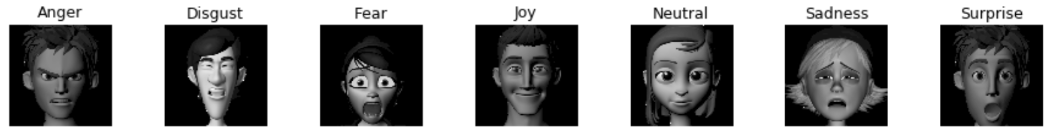
\includegraphics[width=\textwidth,height=2.5cm]{animatedface.png}
      \caption{Animated facial expression dataset.}
      \label{appendix:face-ds}
    \end{center}
\end{figure}

\begin{figure}[H]
    \begin{center}
      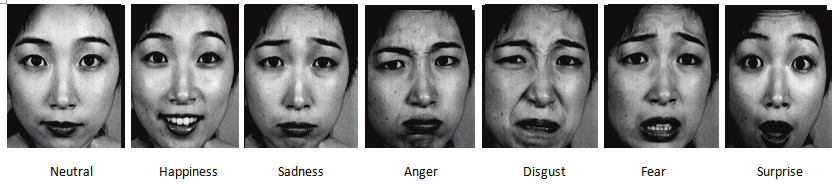
\includegraphics[width=\textwidth,height=2.5cm]{jpwomen.jpg}
      \caption{Japanese female facial expression dataset.}
      \label{appendix:jap-ds}
    \end{center}
\end{figure}

%\end{appendices}

\end{document}
